%!TEX TS-program = xelatex
%!TEX encoding = UTF-8 Unicode

\documentclass[11pt,tikz,border=1]{standalone}
\usetikzlibrary{positioning}

\begin{document}
  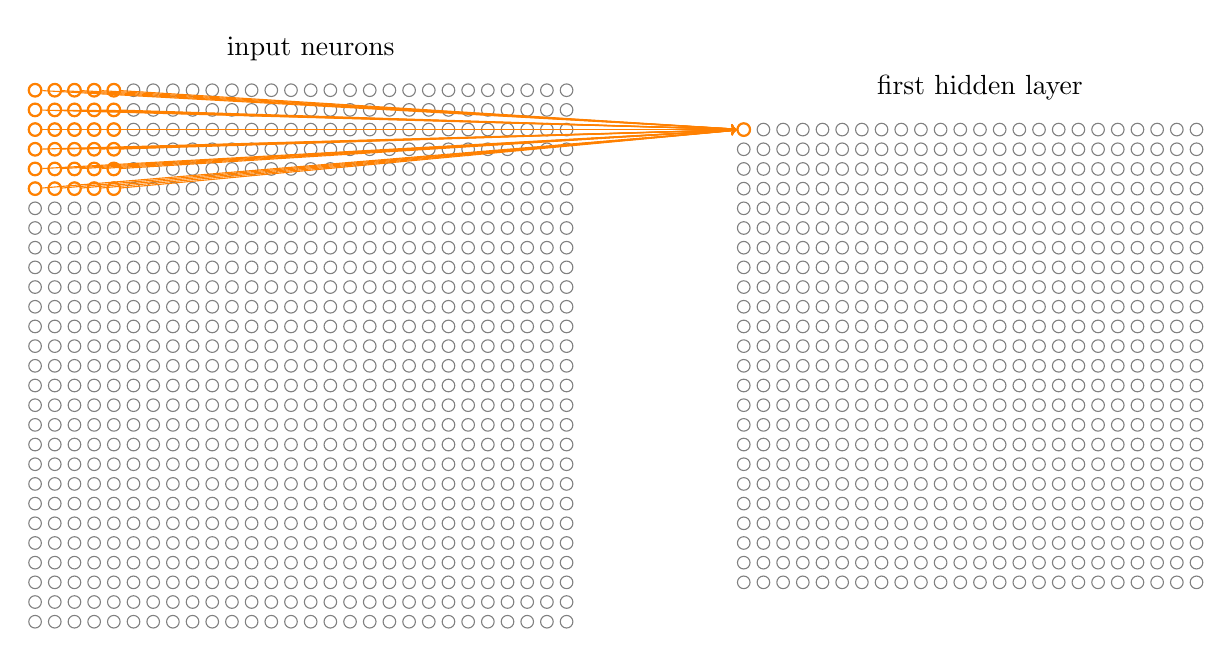
\begin{tikzpicture}[
    neuron/.style={circle,draw,inner sep=0pt,minimum size=1.6mm}
    ]

    \foreach \x in {0,...,27}
      \foreach \y in {0,...,27}
        \node (x\x y\y) [neuron,gray] at (\x * 0.25,\y * 0.25) {};

    \node [above] at (3.5,7) {input neurons};

    \foreach \x in {0,...,23}
      \foreach \y in {0,...,23}
        \node (m\x n\y) [neuron,gray] at (\x * 0.25 + 9, \y * 0.25 + 0.5) {};

    \node [above] at (12, 6.5) {first hidden layer};

    \node(hidden) [neuron,orange,thick] at (m0n23) {};

    \foreach \x in {0,...,4}
      \foreach \y in {22,23,...,27}
        {\node (a\x b\y) [neuron,orange,thick] at (\x * 0.25,\y * 0.25) {};
          \draw[->,orange] (a\x b\y) to (hidden);
        }

  \end{tikzpicture} 
\end{document}
